
\section{Extended Per-Task Results}
\label{app:per_task}

Table~\ref{tab:per_task} reports per-task mean CAR across seeds for each condition. Seven tasks achieve CAR $\geq$ 0.92 under Vanilla, while three physically constrained tasks (T3, T5, T6) fall below 0.58. The overall CAR differences reported in the main text are dominated by these three hard tasks, which average 0.342 compared to 0.968 for the seven non-hard tasks.

\begin{table}[h]
\centering
\caption{Per-task mean CAR across seeds (50 rollouts per seed, v1 code). This table reports v1 codebase results retained for completeness; all main analyses use v2 data (Table~\ref{tab:main_results}). All conditions use 3 seeds except Depth (4). Detach+LN per-task uses 2 seeds (s1, s2; s0 lacks per-task breakdown).}
\label{tab:per_task}
\begin{tabular}{clccccccc}
\toprule
 & & \multicolumn{7}{c}{Mean CAR by Condition} \\
\cmidrule(lr){3-9}
Task & Diff. & Vanilla & Full OCC & Random & Detach & Det+LN & Depth & Cut@35K \\
\midrule
T0 & Easy  & 0.98 & 0.98 & 0.99 & 0.97 & 0.97 & 0.99 & 0.98 \\
T1 & Easy  & 0.92 & 0.93 & 0.99 & 0.89 & 0.78 & 0.93 & 0.95 \\
T2 & Easy  & 0.92 & 0.93 & 0.94 & 0.93 & 0.90 & 0.90 & 0.94 \\
T3 & Hard  & 0.38 & 0.37 & 0.31 & \textbf{0.11} & 0.44 & 0.50 & 0.55 \\
T4 & Med   & 0.98 & 0.99 & 0.95 & 0.98 & 0.96 & 0.92 & 0.97 \\
T5 & Hard  & 0.07 & 0.17 & 0.23 & \textbf{0.05} & 0.12 & 0.08 & 0.04 \\
T6 & Hard  & 0.57 & 0.61 & 0.55 & 0.56 & 0.36 & 0.54 & 0.38 \\
T7 & Easy  & 0.97 & 0.99 & 0.95 & 0.98 & 1.00 & 0.96 & 0.98 \\
T8 & Easy  & 1.00 & 1.00 & 1.00 & 0.99 & 0.99 & 0.99 & 0.99 \\
T9 & Easy  & 1.00 & 0.99 & 0.99 & 1.00 & 1.00 & 1.00 & 1.00 \\
\midrule
\multicolumn{2}{l}{Overall} & 0.780 & 0.797 & 0.789 & 0.746 & 0.765 & 0.780 & 0.779 \\
\bottomrule
\end{tabular}
\end{table}

\textbf{Ceiling effects.} On the seven non-hard tasks (T0--T2, T4, T7--T9), most conditions achieve CAR $\geq$ 0.89, with isolated exceptions (e.g., Detach+LN T1 ${=}$ 0.78), leaving minimal room for auxiliary training to improve performance. The obstacle is spatially separated from the manipulation path in these tasks.

\textbf{Hard task patterns.} On Task~5 (Vanilla CAR 0.07), gradient-flow conditions (Random OCC 0.23, Full OCC 0.17) exceed Vanilla and Detach (0.05), but all values remain below 0.23. Cutoff@35K achieves the highest T3 CAR (0.55) but the lowest T5 CAR (0.04), which illustrates task-specific temporal sensitivity. Depth exhibits high cross-seed variance on hard tasks (T3 range: 0.20--0.78; T6 range: 0.16--0.84), consistent with auxiliary supervision increasing seed sensitivity.

\section{Training Details}
\label{app:training}

\begin{table}[h]
\centering
\caption{Training hyperparameters.}
\begin{tabular}{ll}
\toprule
Parameter & Value \\
\midrule
Base model & OpenVLA-7B~\cite{kim2024openvla} \\
Fine-tuning recipe & OFT~\cite{kim2025oft} \\
Vision encoders & DINOv2 (1024-d) + SigLIP (1152-d) \\
Patch token dim. & 2176 (concatenated) \\
LoRA rank / $\alpha$ & 32 / 16 \\
LoRA trainable params & 110.8M (1.45\% of 7.65B) \\
Optimizer & AdamW (weight decay 0.01) \\
Batch size & 8 \\
Learning rate & $5 \times 10^{-4}$ (constant) \\
Training steps & 50{,}000 \\
Aux.\ loss weight $\lambda_0$ & 0.01 \\
Aux.\ loss decay & $\exp(-t / 50{,}000)$ \\
BEV grid resolution & $64 \times 64$ \\
Focal loss $\alpha$ / $\gamma$ & 0.25 / 2.0 \\
Depth loss & Smooth-L1 \\
Aux.\ head parameters & 1.2M \\
Hardware & NVIDIA RTX PRO 6000 (96\,GB) \\
Wall time per run & $\sim$12.9 hours \\
\bottomrule
\end{tabular}
\end{table}

\textbf{Evaluation protocol.} Each condition uses 3+ seeds (Depth uses 4; Cutoff@15K, Cutoff@25K, and Reverse Cutoff use 2; Cutoff@45K uses 1) with 50 rollouts per task per seed (500 episodes per seed). A collision is registered when the L1 displacement of the obstacle's \texttt{body\_xpos} exceeds $10^{-3}$. Bootstrap 95\% CIs are computed via 10{,}000 resamples (percentile method).

\textbf{Statistical tests.} Pairwise comparisons against Vanilla use two-tailed permutation tests on per-seed mean CARs with Hedges' $g$ (bias-corrected for small samples) for effect size. With $n{=}3$ seeds, statistical power is limited; we report $p$-values and effect sizes for transparency.
\textbf{CKA analysis.} Centered Kernel Alignment~\cite{kornblith2019similarity} measures representational similarity between fine-tuned and pretrained encoder features. We extract patch token activations from the final layer of DINOv2 and SigLIP for 1{,}000 validation images, compute linear CKA per layer, and report the mean across layers. Higher CKA indicates better preservation of pretrained representations.

\textbf{Cutoff implementation.} As described in Section~\ref{sec:ablation}, setting $\lambda(t){=}0$ does not disable the auxiliary head's forward pass; the post-cutoff phase operates in Detach mode with BatchNorm statistics continuing to update (see the Cutoff description therein for details).

\section{Extended Analysis}

% Figure~\ref{fig:gradient_analysis} is in the main text (Results, Gradient Dynamics subsection).

The Detach+LN ablation replaces BatchNorm2d with LayerNorm in the auxiliary head while retaining \texttt{stop\_gradient}. Under v1 (3 seeds), Detach+LN achieves CAR $0.765 \pm 0.023$; under v2 ($n{=}3$), Detach+LN achieves $0.802 \pm 0.024$ (Table~\ref{tab:main_results}), the highest factorial cell mean ($\Delta{=}+5.7$\,pp vs.\ Vanilla, $g{=}+1.89$). This confirms the additive main effects: both detaching gradient flow and using LN independently improve safety.

\textbf{Per-layer gradient analysis.} Figure~\ref{fig:per_layer_combined} decomposes auxiliary gradient flow into two dimensions: amplitude (top row) and direction (bottom row). The amplitude heatmap (panels a--b) shows that Vanilla, Full OCC, and Random OCC maintain comparable action gradient norms across all layers (warm colors), while Detach shows substantially reduced norms across both encoders (dark). These amplitude results were generated from v1 codebase checkpoints. The v2 gradient analysis (Figure~\ref{fig:gradient_analysis}) confirms that the Detach gradient suppression does not reproduce: Detach and gradient-flow conditions maintain comparable action gradient norms under v2, indicating the v1 suppression was a code-path artifact (see Appendix~\ref{app:codebase}). The directional analysis (panels c--d) reveals encoder-specific alignment: DINOv2 conflict rates hover near 46\% across all layers while SigLIP late layers (blocks 21--24) drop to 19--25\%, which indicates cooperative gradient alignment in semantically rich layers. Both patterns are identical for Full OCC and Random OCC, which confirms they arise from architectural structure rather than label content. The aggregate conflict rates (Full OCC 45.6\%, Full OCC+LN 45.7\% under v2; Full OCC 44.1\%, Random OCC 43.9\% under v1) fall below the 50\% expected for random vectors because they reflect this mixture of two encoder-specific patterns.

\begin{figure}[h]
\centering
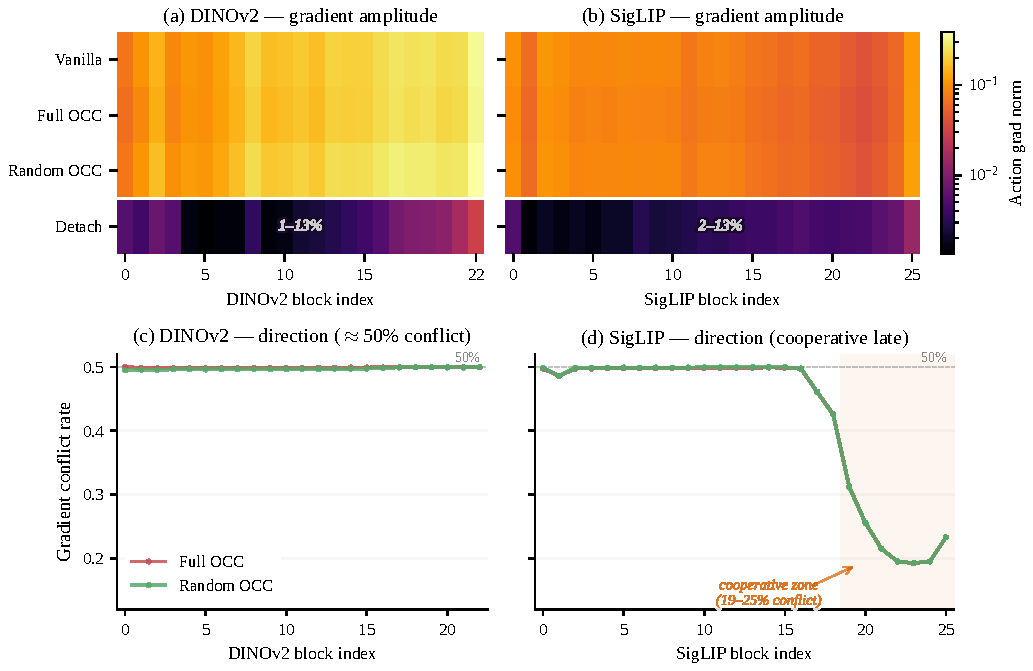
\includegraphics[width=\textwidth]{figures/per_layer_combined.pdf}
\caption{Per-layer gradient analysis decomposed into amplitude and direction (v1 codebase checkpoint, seed 42, 200 batches). \textbf{Top (a--b):} Action gradient norm heatmap (log scale). Gradient-flow conditions (Vanilla, Full OCC, Random OCC) maintain comparable norms; Detach shows substantially reduced norms across all layers, a v1-specific artifact not reproduced under v2 (see Appendix~\ref{app:codebase}). \textbf{Bottom (c--d):} Gradient conflict rate between action and auxiliary losses. DINOv2 maintains $\sim$46\% conflict (near-orthogonal), while SigLIP late layers drop to 19--25\% (cooperative alignment). Both amplitude and directional patterns are identical for Full OCC and Random OCC, confirming architectural rather than label-dependent structure. Directional findings are confirmed under v2; the Detach amplitude suppression (a--b) is a v1 code-path artifact. Conflict rates approach ${\approx}$46\% in early and middle layers; late SigLIP layers show lower conflict rates (${\approx}$25\%), consistent with weak alignment rather than conflict.}
\label{fig:per_layer_combined}
\end{figure}

\subsection{Temporal Dynamics}
\label{app:temporal}
\textbf{Dose-response: gradient flow duration vs.\ CAR (v1 data).} Figure~\ref{fig:dose_response} plots CAR against the number of OCC gradient flow steps for the cutoff series (15K--45K, plus Detach at 0K and Full OCC at 50K; all v1 code). Cutoff@15K (2 seeds, CAR 0.782) clusters near Vanilla (0.780), while Cutoff@25K (2 seeds, 0.724) falls substantially below. Multi-seed conditions (Cutoff@35K and Full OCC) also cluster near the Vanilla baseline. Reverse Cutoff (late 15K) falls below the early-cutoff counterpart at the same gradient flow duration, consistent with the continuity hypothesis. The pattern suggests intermediate cutoff $\approx$ Vanilla rather than a non-monotonic dose-response; the earlier single-seed Cutoff@15K result (0.804) was seed noise.

\begin{figure}[h]
\centering
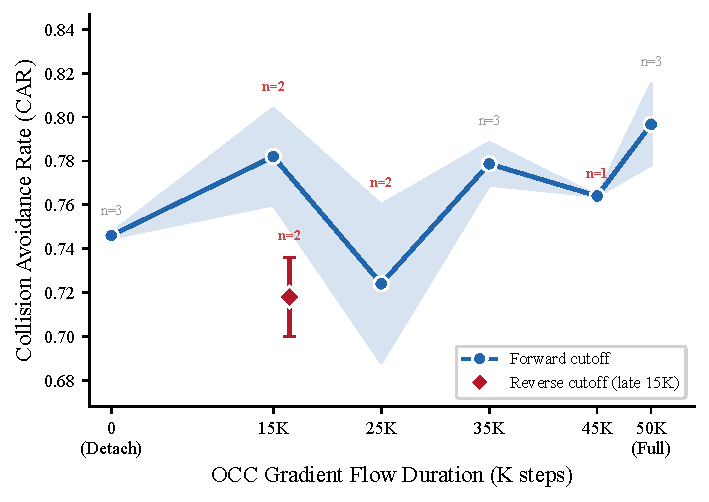
\includegraphics[width=0.75\textwidth]{figures/dose_response.pdf}
\caption{Dose-response: CAR vs.\ OCC gradient flow duration (v1 codebase, all conditions). Filled circles: early-cutoff conditions with all 3 seeds completed; open circles: conditions with $\leq$2 seeds (counts annotated as $n$). Diamond ($\diamond$): Reverse Cutoff (gradient flow restricted to the last 15K steps). Dashed line: Vanilla 3-seed mean (v1); shaded band: $\pm\,$1\,SE. The ``+0.2\%'' annotation marks the Cutoff@15K--Vanilla gap. Intermediate cutoff conditions cluster near Vanilla, while Cutoff@25K and Reverse Cutoff fall substantially below.}
\label{fig:dose_response}
\end{figure}

\section{Additional Observations}
\label{app:additional}

\textbf{Per-task concentration.} Seven of ten tasks achieve CAR $\geq$ 0.92 under Vanilla; overall CAR is dominated by three physically constrained tasks (T3, T5, T6; Section~\ref{app:per_task}). Under the v1 codebase, Detach showed the lowest CAR on these hard tasks (T3: 0.11, T5: 0.05). However, this v1-specific pattern does not replicate under the controlled v2 factorial design (Table~\ref{tab:main_results}), where detaching gradient flow consistently preserves safety (Detach OCC CAR 0.767 vs.\ Vanilla 0.745); the v1 per-task pattern may reflect implementation-specific artifacts rather than a generalizable effect of gradient detachment.

\textbf{Egocentric depth matches Vanilla (v1 data).} Depth (4 seeds) achieves CAR 0.780 $\pm$ 0.039, identical to Vanilla (v1, 0.780), despite providing per-pixel geometric information. Three label types (structured BEV, random binary, egocentric depth) yield comparable CAR when gradient flow is maintained.

\textbf{Temporal dynamics (preliminary, v1 data).} Cutoff@35K (3 seeds) achieves CAR 0.779, statistically indistinguishable from Vanilla (v1, $\Delta = -$0.1\,pp), which confirms that 35K steps of gradient flow fully protects collision avoidance. Surprisingly, Cutoff@25K (0.724, 2 seeds) and Reverse Cutoff (0.718, 2 seeds) fall substantially \emph{below} Vanilla. The most parsimonious explanation: setting the loss weight to zero retains the auxiliary head forward pass, so the post-cutoff period operates in Detach mode; BatchNorm interference acts on representations shaped by gradient flow, without gradient compensation. This is not withdrawal from gradient flow \emph{per se}, but transition into a regime associated with lower safety. Third seeds are in progress; extended analysis in Section~\ref{app:temporal}.

\section{Codebase Sensitivity (v1 vs.\ v2)}
\label{app:codebase}

The five core factorial conditions were retrained under a revised codebase (v2) that fixed a batch-index resume bug affecting cutoff timing and restructured the auxiliary head pipeline (module initialization order, data loading). All model architectures, hyperparameters, LoRA configuration, and evaluation protocols are identical between v1 and v2. The Vanilla baseline (no auxiliary head) is unaffected by these changes, since the revision touches only auxiliary-head code paths.

\textbf{Behavioral shift.} Under v1, Full OCC achieved a mean CAR of 0.797 (3 seeds, per-task Table~\ref{tab:per_task}); under v2, the same condition yields 0.725 $\pm$ 0.064 (Table~\ref{tab:main_results}). Same-seed comparisons show shifts of up to 8.6\,pp, while Vanilla remains stable across codebases ($<$1.5\,pp). This sensitivity is confined to conditions with auxiliary heads and is itself informative: it indicates that auxiliary head training dynamics are fragile with respect to implementation details that would not normally be considered hyperparameters.

\textbf{Gradient analysis shift.} The v1 codebase exhibited a Detach gradient suppression artifact: Detach action-loss gradient norms were only $\sim$4\% of Vanilla norms across all encoder layers. In v2, this suppression disappears entirely (Detach/Vanilla ratio $\approx$ 1.29), indicating that the v1 pattern was a code-path artifact rather than a genuine effect of gradient detachment. The gradient conflict rate also shifted from $\sim$44\% (v1) to $\sim$46\% (v2), with v2 values closer to the theoretical expectation for orthogonal vectors.

\textbf{Effect pattern shift.} Under v1, the normalization $\times$ gradient flow pattern appeared as a crossover ($p{=}0.025$); under v2, both rows slope in the same direction, consistent with two additive main effects rather than an interaction (ANOVA interaction $F{=}0.10$, $p{=}0.763$, $\eta^2{=}0.005$). The crossover pattern in v1 is likely attributable to the Detach gradient suppression artifact described above, which differentially affected BN and LN conditions. All main-text analyses use v2 data exclusively; v1 results are retained in the appendix for completeness and to document the sensitivity.

\textbf{Implication.} The codebase sensitivity reinforces our central finding: auxiliary spatial heads introduce optimization fragility that implementation details can amplify or attenuate. This fragility is a further argument against adding auxiliary spatial heads for safety purposes, since the safety outcome depends on implementation choices that are difficult to specify, reproduce, or audit.

\section{Statistical Power Analysis}
\label{app:stat_power}

The $2{\times}2$ factorial design prioritizes breadth (12 conditions, 5 factors) over per-cell statistical power. With $n{=}3$--$4$ per cell (14 total observations), the design yields medium power for the observed effect sizes. The normalization main effect approaches significance ($p{=}0.060$, $\eta^2{=}0.253$); the gradient flow main effect does not reach significance ($p{=}0.104$) but shows a medium-to-large effect size ($\eta^2{=}0.180$). We report effect sizes as the primary inferential quantity.

The study's evidential strength rests on the consistent direction of both main effects: both BN and LN rows show lower CAR under gradient flow ON than OFF, and both gradient flow conditions show higher CAR under LN than BN. The negligible interaction ($\eta^2{=}0.005$) confirms these effects are additive.

\textbf{Formal $2{\times}2$ ANOVA.} Table~\ref{tab:anova} reports the Type~II factorial analysis ($n{=}3$--$4$ per cell, 14 total observations). The interaction is negligible ($F(1,10){=}0.10$, $p{=}0.763$, $\eta^2{=}0.005$), confirming additive main effects. The normalization main effect approaches significance ($F(1,10){=}4.49$, $p{=}0.060$, $\eta^2{=}0.253$); the gradient flow main effect is medium-sized but non-significant ($F(1,10){=}3.20$, $p{=}0.104$, $\eta^2{=}0.180$). The non-significant gradient flow $p$-value reflects limited per-cell power rather than an absent effect.

\begin{table}[h]
\centering
\caption{$2{\times}2$ factorial ANOVA (Type~II SS). The interaction is negligible; the normalization main effect approaches significance ($p{=}0.060$).}
\label{tab:anova}
\begin{tabular}{lcccc}
\toprule
Source & $F$ & df & $p$ & $\eta^2$ \\
\midrule
Gradient flow (ON vs.\ OFF) & 3.20 & 1,\,10 & 0.104 & 0.180 \\
Normalization (BN vs.\ LN) & 4.49 & 1,\,10 & 0.060 & 0.253 \\
Interaction & 0.10 & 1,\,10 & 0.763 & 0.005 \\
\bottomrule
\end{tabular}
\end{table}

\textbf{Pairwise effect sizes.} Table~\ref{tab:pairwise} reports Hedges' $g$ (bias-corrected) for all factorial cell pairs and versus Vanilla ($n{=}3$--$4$ per cell).

\begin{table}[h]
\centering
\caption{Pairwise Hedges' $g$ (bias-corrected) for factorial cells and Vanilla.}
\label{tab:pairwise}
\small
\begin{tabular}{lc}
\toprule
Comparison & Hedges' $g$ \\
\midrule
Cell~1 (Full OCC BN) vs.\ Cell~2 (Full OCC+LN) & $-$0.88 \\
Cell~1 vs.\ Cell~3 (Detach OCC) & $-$0.78 \\
Cell~1 vs.\ Cell~4 (Detach+LN) & $-$1.28 \\
Cell~2 vs.\ Cell~3 & $+$0.22 \\
Cell~2 vs.\ Cell~4 & $-$0.94 \\
Cell~3 vs.\ Cell~4 & $-$1.24 \\
\addlinespace
Cell~1 vs.\ Vanilla & $-$0.34 \\
Cell~2 vs.\ Vanilla & $+$0.90 \\
Cell~3 vs.\ Vanilla & $+$0.74 \\
Cell~4 vs.\ Vanilla & $+$1.89 \\
\bottomrule
\end{tabular}
\end{table}

\section{Permutation-Based ANOVA}
\label{app:permutation}

To complement the parametric $F$-test (Table~\ref{tab:anova}), we conduct a permutation-based ANOVA~\cite{anderson2001permanova} that makes no distributional assumptions. Following standard practice for factorial designs~\cite{montgomery2017doe}, we use the Type~II $F$-statistic as the test statistic and permute the 14 per-seed CAR values across all cells (10{,}000 permutations). The permutation $p$-value is the proportion of permuted $F$-statistics $\geq$ the observed value.

\begin{table}[h]
\centering
\caption{Permutation-based ANOVA for the $2{\times}2$ factorial (10{,}000 permutations). Both main effects are significant or near-significant; the interaction remains negligible.}
\label{tab:permanova}
\begin{tabular}{lccc}
\toprule
Source & $p_\text{parametric}$ & $p_\text{perm}$ & $\eta^2$ \\
\midrule
Gradient flow (ON vs.\ OFF) & 0.104 & 0.090 & 0.180 \\
Normalization (BN vs.\ LN) & 0.060 & 0.041 & 0.253 \\
Interaction & 0.763 & 0.794 & 0.005 \\
\bottomrule
\end{tabular}
\end{table}

The permutation test yields stronger evidence for the normalization main effect ($p_\text{perm}{=}0.041$, significant at $\alpha{=}0.05$) than the parametric $F$-test ($p{=}0.060$), consistent with the parametric test being conservative for small, non-normal samples. The gradient flow effect does not reach significance under permutation ($p_\text{perm}{=}0.090$) but retains a large effect size ($\eta^2{=}0.180$). The interaction remains negligible ($p_\text{perm}{=}0.794$), confirming the additive pattern.

\textbf{Bayesian model comparison.} A BIC-based Bayes Factor~\cite{wagenmakers2007practical} compares the additive model (main effects only) against a model including the interaction term: $\text{BF}_{01}{=}3.5$, providing moderate evidence that the additive model is preferred. The data are $3.5{\times}$ more likely under the no-interaction model, consistent with the negligible frequentist interaction ($\eta^2{=}0.005$).

\textbf{Safety specificity (TSR).} Applying the same $2{\times}2$ ANOVA to Task Success Rate yields no significant effects (gradient $F(1,10){=}0.85$, $p{=}0.380$; normalization $F(1,10){=}1.34$, $p{=}0.274$; interaction $F(1,10){=}1.08$, $p{=}0.322$), confirming that the safety deficit is specific to collision avoidance and does not reflect general task performance degradation.

\textbf{Leave-one-out sensitivity.} Removing each of the 14 observations and recomputing the ANOVA confirms that both effect directions are robust: $F_\text{gradient} \in [1.73, 6.05]$ (always ON ${<}$ OFF) and $F_\text{norm} \in [3.06, 7.91]$ (always BN ${<}$ LN) across all 14 deletions. The Cell~1 outlier ($\text{CAR}{=}0.654$) inflates but does not create the gradient effect (removing it: $F{=}1.73$, direction preserved); removing the highest Cell~1 seed ($0.776$) strengthens both effects to significance ($p_\text{gradient}{=}0.036$, $p_\text{norm}{=}0.020$), indicating that the reported effects are conservative.

\textbf{Variance heterogeneity.} Levene's test (Brown--Forsythe) does not reject variance homogeneity ($W{=}0.71$, $p{=}0.57$), though the test has limited power at these sample sizes ($n{=}3$--$4$ per cell) and Cell~1 exhibits $5$--$7{\times}$ the variance of other cells ($\sigma^2{=}0.0041$ vs.\ $0.0006$--$0.0007$ for other cells). Welch-corrected marginal tests yield $p{=}0.204$ (gradient) and $p{=}0.104$ (normalization); the attenuation relative to the permutation ANOVA reflects Cell~1's inflated variance entering the standard error. Both effect directions remain consistent under all corrections.

\section{Per-Task Factorial Analysis}
\label{app:per_task_factorial}

The three physically constrained tasks (T3: \texttt{cookie\_box}, T5: \texttt{ramekin}, T6: \texttt{next\_to\_cookie\_box}) show disproportionately large normalization effects under the v2 factorial design.

\textbf{Normalization effect amplification.} The LN advantage over BN averages $+6.9$\,pp on constrained tasks versus $+1.7$\,pp on easy tasks, an approximately $4{\times}$ amplification. All three constrained tasks show positive LN$-$BN differences: T6 ($+9.0$\,pp), T5 ($+7.7$\,pp), T3 ($+4.0$\,pp). The gradient flow effect, by contrast, does not concentrate on constrained tasks ($-1.6$\,pp hard vs.\ $-3.0$\,pp easy), indicating that the two effects have distinct per-task profiles.

\textbf{Cell~1 instability on constrained tasks.} Cell~1 (BN + gradient ON) exhibits $2.4{\times}$ higher cross-seed standard deviation on constrained tasks (mean $\sigma{=}0.217$) than on easy tasks ($\sigma{=}0.092$), consistent with the BN instability mechanism being most consequential where safety margins are thinnest.

\begin{table}[h]
\centering
\caption{Per-task normalization effect by task difficulty (v2 data, seed-weighted means). The LN advantage amplifies ${\approx}4{\times}$ on physically constrained tasks. T4 excluded (medium difficulty).}
\label{tab:per_task_norm}
\small
\begin{tabular}{lccc}
\toprule
Task Group & BN & LN & $\Delta$(LN$-$BN) \\
\midrule
Hard (T3, T5, T6) & $0.288$ & $0.357$ & $+6.9$\,pp \\
Easy (T0--T2, T7--T9) & $0.945$ & $0.962$ & $+1.7$\,pp \\
\bottomrule
\end{tabular}
\end{table}

% Limitations moved to main text
